\documentclass{ctexart}
\usepackage[T1]{fontenc}
\usepackage[a4paper,top=1.5cm,bottom=1.5cm,left=2cm,right=2cm,marginparwidth=1.75cm]{geometry}
\usepackage[fleqn]{amsmath}
\usepackage{mathtools}
\usepackage{tikz}
\usepackage{booktabs}
\usepackage{caption}
\usepackage{outlines}
\usepackage{graphicx}
\usepackage{float}
\usepackage{amsthm}
\usepackage{tabularray}
\usepackage{minted}
\usepackage[colorlinks=false, allcolors=blue]{hyperref}
\usepackage{cleveref}
\usepackage{wrapfig}
\usetikzlibrary{automata,positioning}
\renewcommand{\tableautorefname}{表}
\DeclarePairedDelimiter{\set}{\{}{\}}
\DeclarePairedDelimiter{\paren}{(}{)}
\graphicspath{ {./images/} }

\newcounter{fullrefcounter}
\newcommand*{\fullref}[1]{%
\addtocounter{fullrefcounter}{1}%
\label{--ref-\thefullrefcounter}%
\ifthenelse{\equal{\getpagerefnumber{--ref-\thefullrefcounter}}{\getpagerefnumber{#1}}}
  {
    \hyperref[{#1}]{\Cref*{#1} \nameref*{#1}}
  }
  {% false case
    \hyperref[{#1}]{第 \pageref*{#1} 页 \Cref*{#1} \nameref*{#1}}
  }
}
\newcommand*{\tto}[0]{\Rightarrow}
\newcommand*{\ffrom}[0]{\Leftarrow}
\allowdisplaybreaks
\title{编译原理作业}
\author{卢雨轩 19071125}
% \date{\today}
\ctexset{
    section = {
        titleformat = \raggedright,
        name = {,},
        number = \chinese{section}、
    },
    paragraph = {
        runin = false
    },
    today = small,
    figurename = 图,
    contentsname = 目录,
    tablename = 表,
}

\begin{document}

\maketitle

\begin{outline}
    \1[14.] 给定文法如下,用自然语言描述他们定义的语言
        \2[(1)] $\begin{cases}
            A \to aaA | aaB \\
            B \to Bcc | D\#cc \\
            D \to bbbD | \# \\
        \end{cases}$  \\
        该语言由以下部分顺序连接组成:
        \begin{enumerate}
            \item 偶数个a,至少2个
            \item 3的倍数个b,至少0个
            \item 2个\#
            \item 偶数个c,至少2个
        \end{enumerate}
        \2[(2)] $\begin{cases}
            A \to 0B | 1B | 2B \\
            B \to 0C | 1C | 2C \\
            C \to 0D  1D | 2D | 0 | 1 | 2 \\
            D \to 0B | 1B | 2B 
        \end{cases}$ \\
        长度为3的倍数的、由0,1,2组成的非空串
        \2[(3)] $\begin{cases}
            A \to 0B | 1B | 2B \\
            B \to 0C | 1B | 2B \\
            C \to 0E | 1D | 2D | 0 | 1 | 2 \\
            D \to 0C | 1B | 2B \\
            E \to 0E | 1D | 2D | 0 | 1 | 2
        \end{cases}$ \\
        可化简为:$\begin{cases}
            A \to 0B | 1B | 2B \\
            B \to 0C | 1B | 2B \\
            C \to 0C | 1B | 2B | 0 | 1 | 2 \\
        \end{cases}$,所以是由0,1,2组成的、长度至少为3、倒数第二位为0的串。
        \2[(4)] $\begin{cases}
            S \to aB | bA \\
            A \to a | aS | BAA \\
            B \to b | bS | ABB \\
        \end{cases}$
        相同数量的a和b构成的非空串。
    \1[16.]
        \2[] 最右推导: \\
        $\begin{aligned}
            A &\tto B = E \\
              &\tto B = COD  \\
              &\tto B = COm[1]  \\
              &\tto B = C+m[1]  \\
              &\tto B = b+m[1]  \\
              &\tto D=b+m[1] \\
              &\tto m[2]=b+m[1]
        \end{aligned}$ 

        \begin{minipage}{.45\linewidth}
            \2[]最左归约: \\
            $\begin{aligned}
                m[2]=b+m[1] & \ffrom D = b+m[1] \\
                &\ffrom B = b+m[1]  \\
                &\ffrom B = C+m[1]  \\
                &\ffrom B = COm[1]  \\
                &\ffrom B = COD  \\
                &\ffrom B = E \\
                &\ffrom A \\
            \end{aligned}$
        \end{minipage}
        \begin{minipage}{.45\linewidth}
            \2[] 语法树: \\
            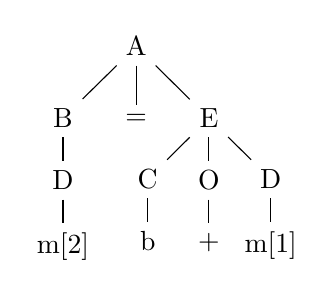
\begin{tikzpicture}
                \node (r) {A};
                \node [below left=.6cm of r] (b) {B};
                \node [below=.5cm of r] (=) {=};
                \node [below right=.6cm of r] (e) {E};
                \node [below=.3cm of b] (d1) {D};
                \node [below left=.4cm of e] (c) {C};
                \node [below=.3cm of e] (o) {O};
                \node [below right=.4cm of e] (d2) {D};
                \node [below=.3cm of d1] (m1) {m[2]};
                \node [below=.3cm of c] (b2) {b};
                \node [below=.3cm of o] (+) {+};
                \node [below=.3cm of d2] (m2) {m[1]};
                \draw (r) -- (b);
                \draw (r) -- (=);
                \draw (r) -- (e);
                \draw (b) -- (d1);
                \draw (d1) -- (m1);
                \draw (e) -- (c);
                \draw (e) -- (o);
                \draw (e) -- (d2);
                \draw (c) -- (b2);
                \draw (d2) -- (m2);
                \draw (o) -- (+);
            \end{tikzpicture}
        \end{minipage}
        \2[] 短语:\\
            $m[2], b, +, m[1],  b+m[1], m[2] = b+m[1]$
        \2[] 直接短语:\\
            $m[2], b, +, m[1]$
        \2[] 句柄:\\
            $m[2]$
    \1[17.]
        \2[] 最右推导:\\
        \begin{align*}
            E &\tto T \\
              &\tto T * F \\
              &\tto T * P \\
              &\tto T * (E)  \\
              &\tto T * (E+T) \\
              &\tto T * (E+F) \\
              &\tto T * (E+P)  \\
              &\tto T * (E+c) \\
              &\tto T * (T+c) \\
              &\tto T * (F+c) \\
              &\tto T * (P+c) \\
              &\tto T * (id + c) \\
              &\tto F * (id + c) \\
              &\tto P * (id + c) \\
              &\tto (E) * (id + c) \\
              &\tto (E+T) * (id + c) \\
              &\tto (E+P) * (id + c) \\
              &\tto (E+F) * (id + c) \\
              &\tto (E+id) * (id + c) \\
              &\tto (T+id) * (id + c) \\
              &\tto (P+id) * (id + c) \\
              &\tto (F+id) * (id + c) \\
              &\tto (c+id) * (id + c)
        \end{align*}
        \begin{minipage}[t]{.45\textwidth}
            \2[] 最左归约: \\
        \begin{align*}
            (c+id) * (id + c) &\ffrom (F+id) * (id + c) \\
              &\ffrom (P+id) * (id + c) \\
              &\ffrom (T+id) * (id + c) \\
              &\ffrom (E+id) * (id + c) \\
              &\ffrom (E+F) * (id + c) \\
              &\ffrom (E+P) * (id + c) \\
              &\ffrom (E+T) * (id + c) \\
              &\ffrom (E) * (id + c) \\
              &\ffrom P * (id + c) \\
              &\ffrom F * (id + c) \\
              &\ffrom T * (id + c) \\
              &\ffrom T * (P+c) \\
              &\ffrom T * (F+c) \\
              &\ffrom T * (T+c) \\
              &\ffrom T * (E+c) \\
              &\ffrom T * (E+P)  \\
              &\ffrom T * (E+F) \\
              &\ffrom T * (E+T) \\
              &\ffrom T * (E)  \\
              &\ffrom T * P \\
              &\ffrom T * F \\
              &\ffrom T \\
              &\ffrom E \\
        \end{align*}
        \end{minipage}
        \begin{minipage}[t]{.45\textwidth}
            \2[] 语法树: \\
        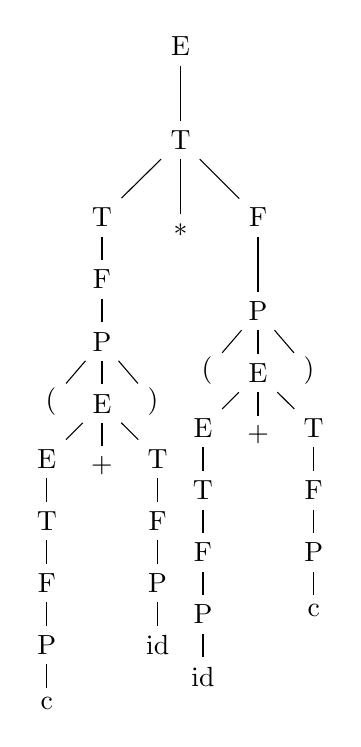
\begin{tikzpicture}
            \node (e0) {E};
            \node (t0) [below=.7cm of e0] {T};
            \node (t1) [below left = .7cm of t0] {T};
            \node (*) [below = .7cm of t0] {*};
            \node (f0) [below right= .7cm of t0] {F};
            \node (p0) [below= .7cm of f0] {P};
            \node (p1) [below left= .3cm of p0] {(};
            \node (e1) [below= .3cm of p0] {E};
            \node (p2) [below right= .3cm of p0] {)};
            \node (e2) [below left= .3cm of e1] {E};
            \node (+) [below= .3cm of e1] {+};
            \node (t2) [below right= .3cm of e1] {T};
            \node (t3) [below= .3cm of e2] {T};
            \node (f3) [below= .3cm of t3] {F};
            \node (p3) [below= .3cm of f3] {P};
            \node (id3) [below= .3cm of p3] {id};
            \node (f4) [below= .3cm of t2] {F};
            \node (p4) [below= .3cm of f4] {P};
            \node (c4) [below= .3cm of p4] {c};

            \draw (e0) -- (t0);
            \draw (t0) -- (t1);
            \draw (t0) -- (*);
            \draw (t0) -- (f0);
            \draw (f0) -- (p0);
            \draw (p0) -- (p1);
            \draw (p0) -- (e1);
            \draw (p0) -- (p2);
            \draw (e1) -- (e2);
            \draw (e1) -- (+);
            \draw (e1) -- (t2);
            \draw (t2) -- (f4);
            \draw (f4) -- (p4);
            \draw (p4) -- (c4);
            \draw (e2) -- (t3);
            \draw (t3) -- (f3);
            \draw (f3) -- (p3);
            \draw (p3) -- (id3);

            
            \node (f1) [below= .3cm of t1] {F};
            \node (p-1) [below= .3cm of f1] {P};
            \node (p44) [below left= .3cm of p-1] {(};
            \node (e1) [below= .3cm of p-1] {E};
            \node (p45) [below right= .3cm of p-1] {)};

            \draw (t1) -- (f1);
            \draw (f1) -- (p-1);
            \draw (p-1) -- (p44);
            \draw (p-1) -- (e1);
            \draw (p-1) -- (p45);

            
            \node (e2) [below left= .3cm of e1] {E};
            \node (+) [below= .3cm of e1] {+};
            \node (t2) [below right= .3cm of e1] {T};
            \node (t3) [below= .3cm of e2] {T};
            \node (f3) [below= .3cm of t3] {F};
            \node (p3) [below= .3cm of f3] {P};
            \node (id3) [below= .3cm of p3] {c};
            \node (f4) [below= .3cm of t2] {F};
            \node (p4) [below= .3cm of f4] {P};
            \node (c4) [below= .3cm of p4] {id};


            \draw (e1) -- (e2);
            \draw (e1) -- (+);
            \draw (e1) -- (t2);
            \draw (t2) -- (f4);
            \draw (f4) -- (p4);
            \draw (p4) -- (c4);
            \draw (e2) -- (t3);
            \draw (t3) -- (f3);
            \draw (f3) -- (p3);
            \draw (p3) -- (id3);
        \end{tikzpicture}
        \end{minipage}
\end{outline}

\end{document}
